\chapter{Datamodellering in Cassandra}
\label{ch:cassandra_modelling}
\section{Primaire sleutel}
Binnen de primaire sleutel in Cassandra worden de partitiekolommen (\ref{partition_key}) en clusteringkolommen (\ref{clustering_key}) vastgelegd voor een tabel.
In tegenstelling tot relationele databases wordt de primaire sleutel hier niet gebruikt als unieke sleutel voor de rij, maar om snel te weten te komen waar de data zich binnen de cluster bevindt \citep{kan2014cassandra}.
Als een tabel slechts één kolom heeft als primaire sleutel, dan is deze kolom meteen ook de partitiekolom en zijn er geen clusteringkolommen.

Door het feit dat de primaire sleutel in Cassandra niet uniek hoeft te zijn, gedragen het INSERT commando en het UPDATE commando zich op een identieke wijze.
Een nadeel hiervan is dat er geen waarschuwing weergegeven wordt als een rij overschreven zou worden.
Omdat dit veelal ongewenst gedrag is binnen applicaties komt men al snel terecht bij een samengestelde primaire sleutel, een primaire sleutel uit verschillende kolommen.

\section{Partitiekolom}
\label{partition_key}
Het eerste deel van de primaire sleutel bestaat uit de partitiekolommen.
Het doel van deze partitiekolommen is om de data gebalanceerd over alle nodes te spreiden.
Op deze manier kan de fysieke locatie van de data ook snel achterhaald worden \citep{kan2014cassandra}.

Bij het kiezen van de partitiekolommen dient men met een aantal zaken rekening te houden om de data evenwichtig over alle nodes te spreiden, maar er is slechts één fysische restrictie.
Iedere rij kan slechts 2 miljard kolommen bevatten \citep{McFadin2013Timeseries}.
In de meeste gevallen is dit ruim voldoende.
Tijdsreeksen vormen hier een uitzondering op.
Deze reeksen kunnen al gauw miljarden entries bevatten.
Hier is het dus zeer belangrijk om  goede partitiekolommen te kiezen of men komt hier al snel in de problemen.

\section{Clusteringkolom}
\label{clustering_key}
Het laatste deel van de primaire sleutel bestaat uit de clusteringkolommen.
Deze bepalen de volgorde van de data op de fysieke media \citep{strickland2014availability}.
De clusteringkolommen hebben echter geen invloed op de fysieke locatie van de data binnen de cluster.
Toch zullen ze een belangrijke invloed hebben op welke query's uitgevoerd kunnen worden.

\section{De WHERE clausule}
Zoals \cite{Lerer2015Where} aanhaalt is één van de grootste verschillen tussen CQL en SQL de WHERE clausule.
In SQL kent de WHERE clausule geen restricties.
Bij CQL is dit anders.
Hier worden restricties opgelegd door de partitie en clusteringkolommen.
Eveneens kan er enkel op de partitie- en clusteringkolommen gefilterd worden.
Al deze restricties komen er door de achterliggende architectuur bij Cassandra.

\subsection{Restricties opgelegd door de partitiekolommen}
Een eerste restrictie die wordt opgelegd door de partitiekolommen is dat ofwel alle partitiekolommen worden opgenomen in de WHERE clausule ofwel geen enkele.
Dit is nodig omdat de partitioner anders de hashwaarde niet kan berekenen.
Deze hashwaarde is echter nodig om te weten op welke node de data zich bevindt (zie sectie \ref{sec:partitioner}).

Een volgende restrictie die wordt opgelegd door de partitiekolommen is het feit dat enkel de '=' en IN operator rechtstreeks gebruikt kunnen worden.
Tot Cassandra 2.2 kon de IN operator enkel op de laatste gedefinieerde partitiekolom toegepast worden.

De laatste restrictie die wordt opgelegd door de partitiekolommen heeft te maken met de >, >=, < en <= operators.
Deze zijn enkel rechtstreeks toepasbaar als de partitioner ingesteld is op ByteOrderedPartitioner.
Indien dit niet het geval is moet men een omweg maken via de token functie.
Op het eerste zicht lijkt het gebruik van de token functie minder efficiënt voor het selecteren van data, maar dit weegt niet op tegen de nadelen die ByteOrderedPartitioner heeft op het gebied van de distributie van de data, zoals eerder vermeld werd.
Wel dient hiermee opgepast te worden omdat de operators dan uitgevoerd worden op de tokens en niet rechtstreeks op de data.
Dit levert niet altijd het gewenste resultaat op.

\subsection{Restricties opgelegd door de clusteringkolommen}
Voor de restricties op de clusteringkolommen uitgelegd kunnen worden, moet eerst uitgelegd worden hoe de data in Cassandra binnen een partitie opgeslagen wordt.
Dit zal nu aan de hand van een voorbeeld uitgelegd worden \citep{Lerer2015Where}.
Neem de onderstaande tabel:

\begin{lstlisting}[caption={Layout van de tabel NumberOfTwitterMessages}, label={lst:twitter_messages}]
CREATE TABLE NumberOfTwitterMessages (
  userid bigint, date text, hour int, minute int,
  nrOfTweets int,
  PRIMARY KEY  ((userid, date), hour, minute)
);

\end{lstlisting}

De eerste restrictie wordt hier opgelegd door de manier waarop de data opgeslagen is.
Als men een voorwaarde wil vastleggen voor een clusteringkolom, dan dienen de clusteringkolommen die voor deze komen in de primaire sleutel ook vastgelegd te worden.
Query \ref{lst:queryMulticlusterColWrong1} is dus niet mogelijk voor de tabel ''NumberOfTwitterMessages'' (\ref{lst:twitter_messages}) omdat hier geen restrictie is op het veld ''hour'', terwijl dit voor het veld ''minute'' komt in de primaire sleutel.
Dit is nodig omdat Cassandra de data anders niet efficiënt kan terugvinden.

\begin{lstlisting}[caption={Foutieve query bij meerdere partitiekolommen}, label={lst:queryMulticlusterColWrong1}, language=SQL]
SELECT nrOfTweets FROM NumberOfTwitterMessages
  WHERE userid = 2222
  AND date = '2016-04-25'
  AND minute = 30
;
\end{lstlisting}

Om te zien waarom deze data niet efficiënt opgehaald kan worden met query \ref{lst:queryMulticlusterColWrong1}, moet men kijken naar de manier waarop Cassandra de data opslaat binnen de partities (zie code fragment \ref{lst:data_partitie}).
Hierbij kan men zien dat er in een boomstructuur gewerkt wordt om de data op te slaan.
Als men echter een top in deze boom weglaat (hier het veld ''hour''), kan het pad naar het veld ''nrOfTweets'', het resultaat van de query, niet op een efficiënte manier bepaald worden.

\begin{lstlisting}[caption={Data opslag binnen een partitie}, label={lst:data_partitie}]
{hour: 20 
  {minute: 4 {nrOfTweets: 6}} 
  {minute: 7 {nrOfTweets: 1}}
  {minute: 21 {nrOfTweets: 16}}
...
}
\end{lstlisting}

Tot Cassandra 2.2 was de IN operator enkel toegelaten op de laatste clusteringkolom.
Sinds Cassandra 2.2 is deze restrictie vervallen en kan men zelfs multi-kolom IN restricties opleggen.

De >, >=, < en <= operators zijn ook enkel toegestaan op de laatste clusteringkolom waar een restrictie aan opgelegd is.
Toch is hier een oplossing voor aangezien men deze operators kan toepassen over meerdere kolommen.
Bij deze multi-column slices is het echter wel belangrijk dat de restrictie van de WHERE clausule met dezelfde kolom start.
Zo is query \ref{lst:queryMultiCol1} perfect mogelijk.
Query \ref{lst:queryMultiCol2} is equivalent aan de vorige query, maar hier wordt ook aangetoond dat de multi-column slice met dezelfde kolom moet beginnen.

\begin{lstlisting}[caption={Multi-column slice restrictie}, label={lst:queryMultiCol1}, language=SQL]
SELECT * FROM NumberOfTwitterMessages
  WHERE userid = 2222
  AND date = '2016-04-25'
  AND (hour, minute) >= (12, 30)
  AND (hour, minute) <= (14, 0)
;
\end{lstlisting}

\begin{lstlisting}[caption={De restrictie moet starten met dezelfde kolom}, label={lst:queryMultiCol2}, language=SQL]
SELECT * FROM NumberOfTwitterMessages
  WHERE userid = 2222
  AND date = '2016-04-25'
  AND (hour, minute) >= (12, 30) 
  AND (hour) <= (14)
;
\end{lstlisting}

\section{Doelen bij datamodellering in Cassandra}
Zoals in bovenstaande sectie duidelijk werd, dient er bij Cassandra met heel wat rekening gehouden te worden als men een datamodel creëert.
\cite{Hobbs2015Datamodelling} definieerde wat de doelen zijn bij het opstellen van een datamodel in Cassandra.
Zoals door Hobbs aangegeven wordt, lijkt de querytaal van Cassandra CQL sterk op SQL, maar kan het gebruik ervan zeer verschillend zijn.

Een eerste doel bij het opstellen van een datamodel in Cassandra is om de data evenwichtig over alle nodes te verspreiden.
Dit kan bekomen worden door de partitiekolommen goed te kiezen.
Zoals eerder vermeld is, worden de partitiekolommen bepaald door het eerste deel van de primaire sleutel.

Een tweede doel is om zo weinig mogelijk partitie reads te moeten doen.
Doordat iedere partitie op een andere node kan staan is dit belangrijk.
Als de partities effectief op verschillende nodes staan moeten de afzonderlijke commando's naar elke node apart verstuurd worden en dit zorgt voor overhead.
Het is zelfs zo dat als de data op dezelfde node staat, de partitie reads nog steeds inefficiënt zijn.
Dit komt door de manier waarop Cassandra de rijen opslaat.

Zaken die bij relationele databanken belangrijk zijn zoals het aantal writes en data duplicatie minimaliseren, zijn binnen Cassandra onbelangrijk.
In Cassandra zijn write operaties goedkoop omdat Cassandra hiervoor geoptimaliseerd is.
Denormalisatie en duplicatie van data zijn ook zeer normaal binnen Cassandra.
Dit komt door de architectuur van Cassandra.
Hierbij gaat men ervan uit dat schijfruimte goedkoop is in vergelijking met andere resources zoals CPU, geheugen, netwerk\dots
Verder heeft Cassandra geen JOIN waardoor het ook hoogst inefficiënt en onpraktisch zou zijn om geen duplicate data te hebben.

\section{Datamodel opstellen voor Cassandra}
\cite{Hobbs2015Datamodelling} definieerde niet enkel de doelen van een datamodel in Cassandra, maar haalt ook aan hoe deze gerealiseerd kunnen worden.
Voor men begint aan het opstellen van een datamodel moet al nagedacht worden over de query's die ondersteund moeten worden.
Dit staat in schril contrast met relationele databanken waar het datamodel wordt bepaald door de objecten en hun relaties.

Door na te denken over de te ondersteunen query's kan het aantal partitie reads al drastisch verminderd worden.
Ook dient men rekening te houden met de restricties die de partitie en clusteringkolommen opleggen aan de WHERE clausule.

Voor iedere query zou er slechts één partitie read uitgevoerd mogen worden.
Hiervoor is het belangrijk dat de tabellen geoptimaliseerd zijn voor de reads die uitgevoerd gaan worden.

Een goed voorbeeld waarin alle zaken meteen duidelijk worden, wordt ook gegeven door \cite{Hobbs2015Datamodelling} .
In dit voorbeeld is het de bedoeling om users op het halen volgens hun email of username.
De oplossing voor Cassandra zijn de volgende twee tabellen \ref{lst:GoodExample}:

\begin{lstlisting}[caption={Correcte datamodellering bij Cassandra},label={lst:GoodExample}, language=SQL]
CREATE TABLE users_by_username (
  username text PRIMARY KEY,
  email text,
  birthday timestamp
);

CREATE TABLE users_by_email (
  email text PRIMARY KEY,
  username text,
  birthday timestamp
);
\end{lstlisting}

Bij dit datamodel krijgt iedere user zijn eigen partitie.
Cassandra kan zo de data evenwichtig verdelen over de nodes.
Om een user op te zoeken via een email of username dient slechts één partitie gelezen te worden.

Stel dat men nu zou proberen om redundante data te verminderen, wat in Cassandra geen doel mag zijn, met de volgende tabellen \ref{lst:BadExample}:

\begin{lstlisting}[caption={Foutieve datamodellering bij Cassandra},label={lst:BadExample}, language=SQL]
CREATE TABLE users (
  id uuid PRIMARY KEY,
  username text,
  email text,
  birthday int
);

CREATE TABLE users_by_username (
  username text PRIMARY KEY,
  id uuid
);

CREATE TABLE users_by_email (
  email text PRIMARY KEY,
  id uuid
);
\end{lstlisting}

De data zal met deze tabellen nog steeds evenwichtig gedistribueerd zijn over de nodes, maar nu moet men meer dan één partitie read doen.
Dus door een niet-doel proberen te bereiken is hier een belangrijk doel verloren gegaan.

\section{Datamodel en de hoge snelheid}
\label{sec:highthroughput}
Nu alle concepten van datamodellering duidelijk zijn, kan er ook verklaard worden waarom dit een effect kan hebben op de schrijf- en leessnelheid van Cassandra.
Hiervoor moet men kijken hoe Cassandra de data fysiek opslaat op de nodes, voor de clusteringkolommen werd dit al even kort aangehaald (zie code fragement \ref{lst:data_partitie}).

Als men nu de tabel ''NumberOfTweets'' (\ref{lst:twitter_messages}) er opnieuw bijneemt, weet men dat de partitiekolommen, ''userid'' en ''date'', de node zullen bepalen waarop de data fysiek aanwezig is.
Men mag aannemen dat deze partitiekolommen ervoor zullen zorgen dat de data evenwichtig verspreid wordt over alle nodes.
Door deze evenwichtige verspreiding zullen de query's ook beter verdeeld worden over de nodes.
Hoe het verdelen van de query's in zijn werk gaat, werd reeds uitgelegd bij de snitches (zie sectie \ref{sec_snitch}).
De hoge schrijfsnelheid wordt bekomen doordat de partitioner het werk over alle nodes verdeelt (zie sectie \ref{sec:partitioner}).
Het is dus zo dat hoe beter de data verspreid is over alle nodes, hoe beter het werk verdeeld kan worden over de nodes.
Door een goede verdeling van het werk kunnen veel query's tegelijk uitgevoerd worden.
Het datamodel is verantwoordelijk voor het verspreiden van de data over alle nodes door middel van de partitiekolommen en zo ook rechtstreeks voor het verspreiden van alle query's over alle nodes.

De clusteringkolommen leveren ook een grote bijdrage tot de hoge leessnelheid van Cassandra.
De clusteringkolommen bepalen hoe de data opgeslagen wordt binnen de partitie.
Met een partitie wordt hier gedoeld op data die gegroepeerd is volgens identieke waarden voor de partitiekolommen.
Binnen de partitie worden de clusteringkolommen opgeslagen in een boomstructuur, zoals eerder al vermeld werd.
Een boomstructuur is een structuur die zeer geschikt is om er opzoekingen in te doen.
Cassandra zorgt er ook voor dat de waarden in de lagen van de boom gerangschikt zijn.
Voor de tabel ''NumberOfTwitterMessages'' (\ref{lst:twitter_messages}) kan dit er dan zoals in figuur \ref{fig:physicalClusterCol} uitzien.

\begin{figure}[H]
	\centering
	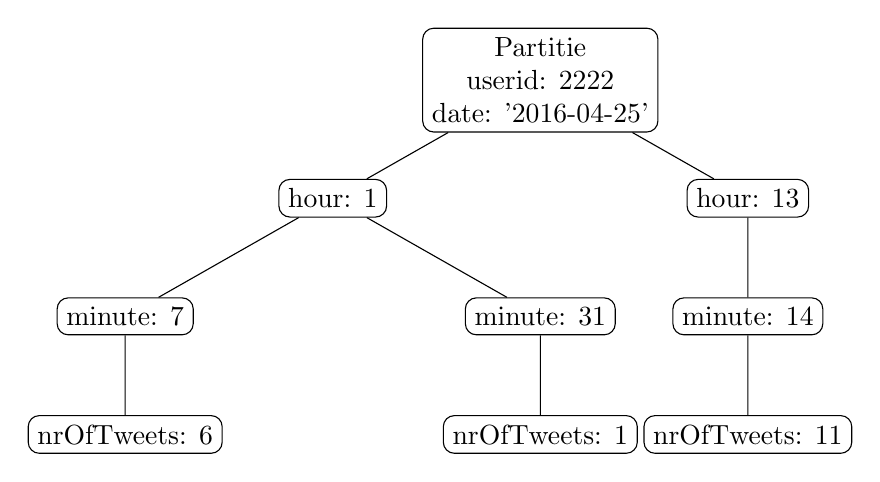
\begin{tikzpicture}[sibling distance=15em,
	every node/.style = {shape=rectangle, rounded corners,
		draw, align=center}]]
	\node {Partitie
		\\userid: 2222
		\\date: '2016-04-25'}
	child { node {hour: 1} 
		child{ node {minute: 7}
			child{node {nrOfTweets: 6}}
		}
		child{ node {minute: 31}
			child{node {nrOfTweets: 1}}
		}
	}
	child { node {hour: 13}
			child{ node {minute: 14}
				child{node {nrOfTweets: 11}}
			}
	}
	;
	\end{tikzpicture}
	\caption{Mogelijke fysieke structuur binnen een partitie}
	\label{fig:physicalClusterCol}
\end{figure}

Door gebruik te maken van deze boomstructuur slaagt Cassandra er dus zeer snel in om de resultaten voor de query's op te halen eenmaal de juiste node en partitie bereikt zijn.
Ook hier is het datamodel verantwoordelijk voor de clusteringkolommen en hiermee dan ook verantwoordelijk voor de efficiëntie waarmee de data opgehaald kan worden.

Het datamodel bepaalt dus hoe efficiënt er gebruik gemaakt wordt van de achterliggende architectuur in Cassandra.
Door het datamodel te optimaliseren kan men hierdoor zeer hoge snelheden bekomen.
Indien men een datamodel maakt dat geen rekening houdt met de query's die uitgevoerd zullen worden, kan men er dus ook voor zorgen dat de snelheden gekelderd worden.